\lstset{language=Haskell}

\title{Обзор методов совместного задания\\
синтаксических анализаторов\\ 
и принтеров\\
для различных языков\\
программирования}

\titlerunning{Обзор методов совместного задания парсеров и принтеров}

\author{Алиев Мирза Али оглы}

\authorrunning{М.Алиев}

\tocauthor{М.Алиев}
\institute{Санкт-Петербургский государственный университет\\
\email{alievmirza@gmail.com}}

\maketitle             

\begin{abstract}
Синтаксический анализ и форматирование (печать)
программного кода являются близкими и связанными задачами.
Соответствующие компоненты языкового процессора должны быть
согласованы между собой, в частности, должно выполняться
свойство обратимости. Для языка Haskell существуют
библиотеки комбинаторов, позволяющие разрабатывать анализаторы и
форматеры вместе, что форсирует выполнение необходимых свойств.
Данная работа посвящена сравнению описанных библиотек. В рамках
практической апробации были разработаны анализаторы и форматеры
для учебного языка L с помощью каждой библиотеки.

\end{abstract}

\section*{Введение}

Во многие языковые процессоры входит синтаксический анализатор. Он получает на вход 
последовательность токенов, сравнивает её с грамматикой исходного языка и, если не 
появилось никаких ошибок, строит древовидную структуру программы, называемую 
синтаксическим деревом (см. риc.~\ref{Code},~\ref{Tree}).

\begin{figure}[h]
  \begin{minipage}[h]{\textwidth}
    \centering
    \begin{lstlisting}[language=C]
    while(a<b){
        printf("a is less than b");
    }
    \end{lstlisting}
    \caption{Код программы.}
    \label{Code}
  \end{minipage}
  \vskip 3mm
  \begin{minipage}[h]{\textwidth}
    \centering
    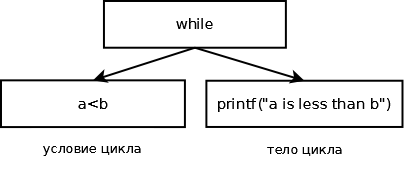
\includegraphics[width=8cm]{Aliev/whileTree.png}
    \caption{Синтаксическое дерево.}
    \label{Tree}
  \end{minipage}
\end{figure}

Помимо синтаксического анализатора языка часто реализуют так называемый pretty-printer, 
который в дальнейшем будет называть принтером, а сам процесс его работы~--- печатью. Он позволяет 
получить текстовое представление программы на основе синтаксического дерева. Однако у программы может 
быть несколько представлений, и то, какой код получится, играет немаловажную роль. На рис.~\ref{nonformatted} 
представлен код неотформатированной программы, на рис.~\ref{formatted} тот же самый код, но уже с добавлением 
отступов, переносов строк, пробелов в определённых местах, что намного облегчает восприятие программы.

\begin{figure}[h]
\centering
\begin{lstlisting}[language=C]
    int foo(int a, int b){while(a<b)
    {printf("a is less than b")
    ;a=a+1;}return a;}
\end{lstlisting}
\caption{Неотформатированная программа}
\label{nonformatted}
\end{figure}

\begin{figure}[h]
\centering
\begin{lstlisting}[language=C]
    int foo(int a, int b)
    {
        while(a<b)
        {
            printf("a is less than b");
            a = a+1;
        }
        return a;
    }    
\end{lstlisting}
\caption{Форматированная программа}
\label{formatted}
\end{figure}

В большинстве случаев синтаксический анализатор и принтер никак не связаны между собой и являются двумя 
разными программами, хотя выполняют они функции, обратные друг к другу, то есть для них можно 
ввести следующий инвариант: пусть имеется синтаксический анализатор 

\lstinputlisting[language=Haskell, firstline=1, lastline=1]{Aliev/printer.hs}

\noindent и принтер

\lstinputlisting[language=Haskell, firstline=2, lastline=2]{Aliev/printer.hs}

Все строки, которые равны с точки зрения синтаксиса языка, будут давать одно и тоже синтаксическое дерево, 
однако по одному и тому же синтаксическому дереву принтер может получить разные строки, отличающиеся, 
например, количеством пробелов как на рис.~\ref{nonformatted} и~\ref{formatted}.
Из этого следует, что композиция синтаксического анализатора и принтера будет тождественной функцией

\lstinputlisting[language=Haskell, firstline=3, lastline=3]{Aliev/printer.hs}

\noindent а обратная композиция не является тождественной:

\lstinputlisting[language=Haskell, firstline=4, lastline=4]{Aliev/printer.hs}

Для разработки синтаксических анализаторов и принтеров на языке Haskell довольно часто используются 
библиотеки и встраиваемые предметно-специфичные языки (Embedded Domain-Specific Languages, EDSLs). Например, 
стандартные библиотеки ghc включают в себя библиотеку Parsec, встроенный синтаксический анализатор DSL~\cite{parsec} 
для синтаксического анализа, а также EDSL для реализации принтеров~\cite{Hughes1995}. Эти библиотеки независимы 
между собой и сложны в реализации, так как от них требуется высокая скорость работы и корректность. 
Все это усложняет соблюдение инварианта принтера и синтаксического анализатора.

Возникает вопрос о совместном задании принтера и синтаксического анализатора, т.е. написание одного
кода, по которому порождаются обе сущности. У этого подхода есть ряд 
положительных качеств. Во-первых, это позволит не реализовывать две схожие программы отдельно. 
Как следствие, сводится к минимуму вероятность появления ошибок,
связанных с их взаимодействием (в том числе соблюдение описанного выше инварианта).
Кроме того, 
такой подход позволит не переносить изменения, сделанные в одном компоненте, на другую. Во-вторых, 
все строки, которые порождаются принтером, должны корректно восприниматься синтаксическим анализатором. 
В-третьих, инвариантность принтера и синтаксического анализатора получается автоматически
за счёт задания их как единой структуры.

В данной работе рассматриваются три статьи, предоставляющие возможности совместного задания 
принтера и синтаксического анализатора для формальных языков~\cite{Rendel,Matsuda,Boespflug}.
Целью работы является обзор существующих статей в данной предметной области, выявление их 
положительных и отрицательных сторон, а именно: как сильно можно варьировать вывод принтера, 
можно ли изменять параметры вывода, например, ширину. Для этих целей на основе каждой статьи 
реализуется синтаксический анализатор и принтер для учебного языка L. На рисунках~\ref{lol1} и~\ref{lol2} 
показаны два различных представления кода в зависимости от того, какая была установлена ширина вывода.

\begin{figure}[h]
  \centering
  \begin{minipage}[h]{0.4\textwidth}
    \begin{lstlisting}[language=C]
printf("a is less than b"); a = b;
    \end{lstlisting}
    \caption{Представление программы при ширине вывода больше 34}
    \label{lol1}
  \end{minipage}
  \hfill
  \begin{minipage}[h]{0.4\textwidth}
    \begin{lstlisting}[language = C]
printf("a is less than b"); 
    a = b;
    \end{lstlisting}
    \caption{Представление программы при ширине вывода меньше 34}
    \label{lol2}
  \end{minipage}
\end{figure}

\section{Обратимые синтаксические описания}

Авторами данного подхода~\cite{Rendel} был разработан EDSL синтаксических описаний (syntax descriptions) 
для объединения синтаксического анализа и печати, основанный на частичных изоморфизмах 
(partial isomorphisms), с помощью которых можно осуществлять обратимые вычисления. 
Авторы предоставляют интерфейс синтаксических описаний как множество классов типов (type classes). 
Также они разработали единые комбинаторы для синтаксического анализа и печати.

Рассмотрим пример. На рис.~\ref{AST} представлен результат обработки строки "\cd{((SK)K)}" на языке 

\begin{verbatim}
   SK : S | K | App SK SK
\end{verbatim}

синтаксическим анализатором.

\begin{figure}[h]
  \centering
  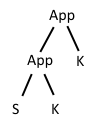
\includegraphics[scale = 0.9]{Aliev/AST.png}
  \caption{Синтаксическое дерево}
  \label{AST}
\end{figure}

Программа, реализующий синтаксический анализатор и принтер выглядит следующим образом (см. рис.~\ref{ppimpl}).

\begin{figure}[h]
\centering
\begin{lstlisting}[language=Haskell]
    parserSK = exp1 where
        exp0 = s <$ tok "S"
           <|> k <$ tok "K" 
           <|> tok "(" *> exp1 <* tok ")"
        exp1 = foldl app <$> exp0 <*> many exp0
        tok k = string k <* spaces    
\end{lstlisting}
\caption{Синтаксический анализатор и принтер}
\label{ppimpl}
\end{figure}

Рассмотрим комбинатор \lstinline{(<$>)}, как если бы он был реализован в библиотеке, 
которая осуществляет лишь синтаксический анализ. Этот комбинатор имел бы тип

\begin{lstlisting}[language=Haskell,mathescape]
   ($\alpha$ -> $\beta$) -> (Parser $\alpha$ -> Parser $\beta$)
\end{lstlisting}

\noindent и позволял бы получить синтаксический анализатор некоторого типа $\beta$, имея 
синтаксический анализатор типа $\alpha$ и функцию из $\alpha$ в $\beta$. Теперь 
рассмотрим этот же комбинатор с точки зрения принтера. Он имел бы тип 

\begin{lstlisting}[language=Haskell,mathescape]
   ($\beta$ -> $\alpha$) -> (Printer $\alpha$ -> Printer $\beta$)
\end{lstlisting}

Как видно, два типа очень похожи, за исключением того, что в одном случае первый аргумент имеет тип $\alpha \rightarrow \beta$, 
а во втором $\beta \rightarrow \alpha$.

Для обобщения комбинаторов для синтаксического анализа и печати авторами вводится понятие \emph{частичного изоморфизма}. 
Заводится конструктор типа данных \lstinline{Iso}, такой, что \lstinline[language=Haskell,mathescape]{Iso $\alpha$ $\beta$}~---
это тип частичного изоморфизма между $\alpha$ и $\beta$:

\begin{lstlisting}[mathescape,language=Haskell]
   data Iso $\alpha$ $\beta$ =
        Iso ($\alpha$ -> Maybe $\beta$) ($\beta$ -> Maybe $\alpha$)
\end{lstlisting}

Слово частичный здесь не случайно, как видно из определения типа в значении \lstinline[language=Haskell,mathescape]{Iso $f$ $g$}
функции $f$ и $g$ по входному параметру могут вернуть \lstinline[language=Haskell]{Nothing}. 

Теперь функции могут быть использованы как ``вперед'', так и в обратную сторону. Например, модифицированный комбинатор 
\lstinline[language=Haskell]{<$>}, выглядящий следующим образом:

\begin{lstlisting}[language=Haskell,mathescape]
   (<$\$$>) :: Syntax $\delta$ => Iso $\alpha$ $\beta$ -> ($\delta\;\alpha$ -> $\delta\;\beta$)
\end{lstlisting}

\noindent выполняет следующие функции: из \lstinline[language=Haskell,mathescape]{$f$ <$\$$> $p$} синтаксический анализатор будет 
использовать функцию $f$ ``вперед'' для того, чтобы конвертировать значения после синтаксического анализа, а принтер будет использовать 
$f$ в обратную сторону перед печатью. Однако не все функции могут быть использованы при частичном изоморфизме, а только те, 
которые могут быть обратимы. Так, для хорошо известной функции свертки

\begin{lstlisting}[mathescape,language=Haskell]
   foldl :: ($\alpha$ -> $\beta$ -> $\alpha$) -> $\alpha$ -> [$\beta$] -> $\alpha$
\end{lstlisting}

авторы реализуют её обратимый вариант

\begin{lstlisting}[mathescape,language=Haskell]
   foldl :: Iso ($\alpha$, $\beta$) $\alpha$ -> Iso($\alpha$, [$\beta$]) $\alpha$
\end{lstlisting}

При этом ``обращеное направление'' функции \lstinline{foldl} даёт функцию \lstinline{unfoldl}.

Всё это позволило авторам разработать интерфейс, который позволяет совместно задать синтаксический анализатор и принтер (см. рис.~\ref{ClassSyntDesc}).

\begin{figure}[ht]
\centering
\begin{lstlisting}[mathescape,language = haskell]
class (IsoFunctor $\delta$, ProductFunctor $\delta$, Alternative $\delta$) 
    => Syntax $\delta$ where
   $(<\$>)$ : Iso $\alpha$ $\beta$ -> $\delta\;\alpha$ -> $\delta\;\beta$
   $(<*>)$  : $\delta\;\alpha$ -> $\delta\;\beta$ -> $\delta$ ($\alpha$, $\beta$)
   $(<|>)$  : $\delta\;\alpha$ -> $\delta\;\alpha$ -> $\delta\;\alpha$
   empty    : $\delta\;\alpha$
   pure     : Eq $\alpha$ => $\alpha$ -> $\delta\;\alpha$
   token    : $\delta$ Char
\end{lstlisting}
\caption{Класс синтаксических дескрипторов}
\label{ClassSyntDesc}
\end{figure}

Дескриптор \lstinline[language=Haskell]{token} связывает символ с самим собой, \lstinline[language=Haskell]{pure x} 
в случае синтаксического анализа возвращает \lstinline[language=Haskell]{x}, не требуя какого-либо ввода, а, в случае 
принтера, отбрасывает значения, равные \lstinline[language=Haskell]{x}. Используя этот интерфейс, можно 
реализовать функцию, которая является и синтаксическим анализатором, и принтером.

Недостатком обозреваемого подхода является невозможность стандартными способами задать 
вариативность принтера в зависимости от ширины вывода. 
Однако при реализации пары принтера и синтаксического анализатора для учебного языка L с использованием
описанной библиотеки было выяснено, что с помощью небольшой обёртки для приведенных
комбинаторов можно построить функцию, дополнительно зависящую от 
булевого флага. Этот флаг позволит в рамках принтера варьировать количество пробелов, переносов строк, отступов.
Ниже представлена часть программы, использующей данный флаг, и пример работы, показывающий
полученную вариативность.

\begin{figure}[ht]
\centering
\begin{lstlisting}[language=Haskell]
optSpace' :: Syntax delta => Bool -> delta ()
optSpace' True  = 
  ignore [()] <$> (many (text "~\textbackslash~n   ") <|> many (text " "))
optSpace' False = 
  ignore [()] <$> (many (text " ") <|> many (text "~\textbackslash~n"))
statement = stm 1 where
  stm 0 = readStm <$> readstm
    <|> write <$> write'
    <|> while <$> while'
    <|> ifExp <$> ifexp
 stm 1 = (seqStm <$> (stm 0 <*> text ";" *> stm 1))
    <|> stm 0
 readstm = keyword "read"
    *> parens (identifier)
 write' = keyword "write"		  
    *> parens (expression)
 while' = keyword "while"
    *> parens (expression) <*> optSpace' False *> (statement)
 ifexp = keyword "if"
   *> optSpace *> parens (expression)
  <*> optSpace *> (statement) 
  <*> optSpace *> keyword "else"  
   *> optSpace *> (statement)	
\end{lstlisting}
\caption{Реализация булевого флага}
\label{boolFlag1}
\end{figure}

При выставлении у функции \lstinline[language=Haskell]{optSpace'} параметра 
\lstinline[language=Haskell]{True} происходит форматирование, как на рис.~\ref{True}, 
а при параметре \lstinline[language=Haskell]{False}~--- как на рис.~\ref{False}

\begin{figure}[h]
  \centering
  \begin{minipage}[h]{0.4\textwidth}
    \begin{lstlisting}[language = C]
    while(1)
       read(x)
    \end{lstlisting}
    \caption{Флаг равен \lstinline[language=Haskell]{True}}
    \label{True}
  \end{minipage}
  \hfill
  \begin{minipage}[h]{0.4\textwidth}
    \begin{lstlisting}[language = C]
    while(1) read(x)
    \end{lstlisting}
    \caption{Флаг равен \lstinline[language=Haskell]{False}}
    \label{False}
  \end{minipage}
\end{figure}


Однако мы стремимся получить вариатиность не от булевого флага, а в зависимости от ширины вывода. 
Для того, чтобы появилась такая возможность, нужно либо придумывать более сложные структуры, 
нежели флаг, либо обернуть получение параметров вывода в монадические вычисления. Однако
остается открытым вопрос, возможно ли это в рамках идеи обратимости.

Одним из несущественных ограничений существующей реализации данного подхода является
использование расширений языка Haskell, на сегодняшний день доступных только в компиляторе
GHC\footnote{\texttt{https://www.haskell.org/ghc/}}.

\section{Обратимые принтеры}

\begin{wrapfigure}[9]{r}[0pt]{.4\textwidth}
\vspace{-.8cm}
\centering
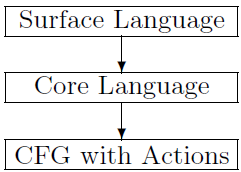
\includegraphics[scale=0.5]{Aliev/FliPprScheme.png}
\caption{Схема работы FliPpr}
\label{FliPpr}
\end{wrapfigure}

В статье~\cite{Matsuda} авторы разработали систему FliPpr для получения синтаксического 
анализатора из принтера. Одним из важных элементов системы FliPpr является язык Surface Language, 
оснащённый комбинаторами библиотеки Вадлера для печати~\cite{WadlerPrinter}, с помощью которого 
реализуется принтер.
Далее программа на языке Surface Language преобразуется
в описание на языке Core Language 
с помощью системы FliPpr. Следующим этапом работы системы является генерация контексно-свободной 
грамматики по полученному описанию на Core Language. В итоге полученная грамматика передается 
парсер-генератору и получается синтаксический анализатор (рис.~\ref{FliPpr}).
Рассмотрим работу систему FliPpr на примере. На рис.~\ref{printer_example} представлен принтер 
для небольшого языка, состоящего из единственного нетерминала
\texttt{E}.
\begin{figure}[h]
\centering
\begin{lstlisting}[language=Haskell]
  -- Language: E :: Sub E E | One
  ppr x = ppr x <+ text "(" <> nil <> ppr x <> nil <> text ")"
  ppr One = text "1"
  ppr (Sub e1 e2) = group (ppr e1 <> 
                    nest 2 (line' <> text "-" <> space' <> 
                            pprP e2))
  pprP x = pprP x <+ text "(" <> nil <> pprP x <> nil <> 
           text ")"
  pprP One = text "1"
  pprP (Sub e1 e2) = text "(" <> nil <> 
                      group (ppr e1 <> 
                        nest 2 (line' <> text "-" <> 
                                space' <> pprP e2
                               )
                            ) <> nil <> 
                     text ")"
  space' = space <+ text ""
  line'  = line <+ text "" 
\end{lstlisting}
\caption{Пример принтера}
\label{printer_example}
\end{figure}

Помимо комбинаторов Вадлера
group и nest \cite{WadlerPrinter}, авторами FliPpr
вводится комбинатор выбора 
\lstinline[language=Haskell]{(<+)} (Biased Choice). Он нужен для того, чтобы синтаксический 
анализатор мог воспринимать не только строчки, которые производит принтер. Принцип действия 
этого комбинатора следующий: когда программа воспринимается как принтер, то выполняется 
действие лишь левого операнда \lstinline[language=Haskell]{(<+)}. Однако с точки зрения 
синтаксического анализатора этот комбинатор интерпретируется как недетерменированный выбор, 
который принимает как левый, так и правый операнд. Например, можно определить количество 
пробелов и переносов строк следующим образом:

\begin{lstlisting}[language=Haskell,mathescape]
  $nil$ = $text$ "" <+ $space$
  $space$ = ($text$ " " <+ $text$ "~\textbackslash~n") <> $nil$
\end{lstlisting}

\noindent где $nil$ позволял бы воспринимать ноль или больше пробелов с переносом строки во 
время синтаксического анализа и получать ноль пробелов во время печати, а  $space$ позволял 
бы воспринимать один или больше пробелов с переносом строки во время синтаксического 
анализа и получать один пробел во время печати. Например, строки вида 

\begin{lstlisting}[language=Haskell]
   1    - 1, (1)-((1)), (1 - (1))
\end{lstlisting} 

\noindent анализируются корректно.

Данный подход получения синтаксического анализатора из принтера основывается на предыдущей работе авторов
об инверсии, основанной на грамматике целевого языка
(grammar-based inversion)~\cite{MatsudaPrew}.
Используя идеи из статьи~\cite{MatsudaPrew}, 
программа на языке Core Language может быть инвертирована для получения контекстно-свободной 
грамматики особого вида (CFG with actions) (см. рис.~\ref{CFGAct}) исходного языка. 
Далее в программе FliPpr авторами используется парсер-генератор, основанный на работе~\cite{Frost} 
для получения синтаксического анализатора. Однако для того, чтобы инверсия была возможна, 
на программу на языке Core Language накладываются ограничения, а именно, программа должна 
быть линейной и ``treeless''~\cite{WadlerDeforest}. Вследствие этих ограничений нельзя 
релизовать хороший принтер с гибкими настройками форматирования, поэтому был разработан 
Surface Language, но уже без вышеуказанных ограничений, дающий возможности хорошей 
печати, а далее с помощью дефорестирования~\cite{WadlerDeforest} и др. программа на языке 
Surface Language переводится в программу на Core Language.

\begin{figure}[h]
\centering
\begin{lstlisting}[language=Haskell,mathescape]
PPr -> Ppr_                      {$\textdollar$ 1}
    | "(" Nil Ppr Nil ")"       {$\textdollar$ 3} 
Ppr_$\rightarrow$ 1             {$\textdollar$ One}
    | Ppr Line' "-" Space' PprP {Sub $\textdollar$1 $\textdollar$5 }
...    
\end{lstlisting}
\caption{Пример CFG with actions}
\label{CFGAct}
\end{figure}

На рисунке~\ref{LFliPpr} представлена часть реализации принтера на яыке Surface Language для учебного 
языка L, которая обрабатывает цикл while.

\begin{figure}[ht]
\centering
\begin{lstlisting}[language=Haskell]
   ppr' i d (ExWhileZ _ x y ) = parensIf (d == L) $ group $ 
       text "while" <> nil <> space' <> ppr 0 R x <> line <> 
       text "do" <> space <> nest 3 (ppr 0 R y);                                                
   parensIf b d = if b then parens d else d ;
   manyParens d = d <+ parens (manyParens d);
   parens d = text "(" <> nest 1 (nil <> d <> nil) <> text ")";
   space = (text " " <+ charOf (spaceChars `butnot` char ' ')) 
           <> nil;
   nil = text "" <+ (charOf spaceChars <> nil);
\end{lstlisting}
\caption{Обработка цикла while для языка L}
\label{LFliPpr}
\end{figure}

Достоинством данного метода является то, что для принтера используются комбинаторы из библиотеки Вадлера. 
Это предоставляет широкие возможности для форматирования, в том числе с использование ширины вывода. 
Также стоит отметить вариативность в плане выбора парсер-генератора. Однако ограничения, которые
накладываются на Core Language, могут в перспективе вызвать ограничения при реализации 
синтаксических анализаторов и принтеров для сложных структур.

\section{``Кассеты''}

В данной статье~\cite{Boespflug} авторы представляют EDSL c семейством обратимых комбинаторов для совместного 
задания синтаксического анализа и печати. Для реализации данного подохода авторы разработали 
тип под названием ``кассета'' (Cassette). Кассета состоит из двух ``треков'', которые представлены функциями:

\begin{lstlisting}[mathescape,language=Haskell]
   data K7 a b c d = 
        K7 { sideA :: a -> b, sideB :: d -> c }
\end{lstlisting}

Кассеты можно склеивать для получения новых:

\begin{lstlisting}[mathescape,language=Haskell]
  (<>) :: K7 b c b' c' -> K7 a b a' b' -> K7 a c a' c'
  $\sim$(K7 f f') <> $\sim$(K7 g g') = K7 (f . g) (g' . f')
\end{lstlisting}

Кассета, которая на стороне А содержит синтаксический анализатор, продуцирующий данные типа $а$, и которая
на стороне B имеет принтер данных типа $а$, называется P/P парой:

\begin{lstlisting}[mathescape,language=Haskell]
  type PP a = forall r r'. K7 (C (a -> r)) (C r) (C (a -> r')) (C r')
\end{lstlisting}

\noindent где конструктор \lstinline[language=Haskell]{C} имеет тип 

\begin{lstlisting}
   type C r = (String -> r) -> String -> r
\end{lstlisting}

С кассетами можно делать следующие действия. Их можно проиграть:

\begin{lstlisting}[mathescape,language=Haskell]
   play :: K7 a b c d -> a -> b
   play csst = sideA csst
\end{lstlisting}

Можно поменять стороны A и B местами:

\begin{lstlisting}[mathescape,language=Haskell]
   flip :: K7 a b c d -> K7 d c b a
   flip (K7 f g) = K7 g f
\end{lstlisting}

Простейший синтаксический анализатор из кассеты получается следующим образом:

\begin{lstlisting}[mathescape,language=Haskell]
   parse :: PP a -> String -> Maybe a
   parse csst = play csst (\_ _ x -> Just x) (const Nothing)
\end{lstlisting}

Если перевернуть кассету, то получится принтер:

\begin{lstlisting}[mathescape,language=Haskell]
   pretty :: PP a -> a -> Maybe String
   pretty csst = play (flip csst) (const Just) (\_ _ -> Nothing) ""
\end{lstlisting}

\begin{figure}[ht]
\centering
\begin{lstlisting}[language=Haskell]
optSpace' ::  Bool -> PP0
optSpace' True  = unshift "~\textbackslash~n   " $ many (satisfy isSpace)
optSpace' False = unshift " " $ many (satisfy isSpace)

stmnt :: PP Stmt
stmnt = 
    seqL -->
      parens (stmnt<> optSpace <> string ";" <> optSpace <> 
              stmnt)
 <|> readL   -->
      string "read" <> parens(ident)
 <|> writeL  -->
      string "write" <> parens(optSpace <> mainExpr <> optSpace)
 <|> whileL  -->
      string "while" <> parens(optSpace <> mainExpr <> optSpace) 
      <> optSpace' True <> optSpace <> stmnt <> optSpace 
 <|> assignL --> 
      ident <> optSpace <> string "=" <> optSpace <> mainExpr  
\end{lstlisting}
\caption{Реализация булевого флага}
\label{boolFlag2}
\end{figure}

Комбинатор \lstinline[language=Haskell]{(<|>)} позволяет выбирать последовательно 
между несколькими кассетами. Если одна из них, например, не может проанализировать 
входную строку, то выбирается следующая кассета:

\begin{lstlisting}[mathescape,language=Haskell]
   (<|>) :: PP a -> PP a -> PP a
   K7 f f' <|> K7 g g' =
     K7 (\k k' s -> f k (\s' -> g k k' s) s)
        (\k k' s x -> f' k (\s' -> g' k k' s) s x)
\end{lstlisting}

Основной особенностью данного подхода является то, что симметричность синтаксического 
анализатора и принтера реализуется с помощью задания их индуктивно (Continuation-passing style, CPS). 
По мнению авторов, такой способ задания комбинатора выбора \lstinline[language=Haskell]{(<|>)} 
показывают лучшие результаты в плане производительности, нежели c помощью методов, описанных 
в первой статье~\cite{Rendel}, где были использованны вложенные кортежи. 

Данный метод никак не позволят варьировать работу принтера в зависимости от ширины вывода. 
Как и в случае с первой статьей, был реализован синтаксический анализатор и принтер с булевым флагом, 
в зависимости от которого продуцировался разный вывод. Ниже представлена часть программы, 
реализующая флаг и результаты работы программы в зависимости от параметра.

\begin{figure}[h]
  \centering
  \begin{minipage}[h]{0.4\textwidth}
    \begin{lstlisting}[language=C]
    while( 1 )
       read(x)
    \end{lstlisting}
    \caption{Флаг равен \lstinline[language=Haskell]{True}}
    \label{True1}
  \end{minipage}
  \hfill
  \begin{minipage}[h]{0.4\textwidth}
    \begin{lstlisting}[language=C]
    while( 1 ) read(x)
    \end{lstlisting}
    \caption{Флаг равен \lstinline[language=Haskell]{False}}
    \label{False1}
  \end{minipage}
\end{figure}

При выставлении у функции \lstinline[language=Haskell]{optSpace'} параметра \lstinline[language=Haskell]{True} 
происходит форматирование, как на рис.~\ref{True1}, а при параметре \lstinline[language=Haskell]{False}~--- как на рис.~\ref{False1}.

\section{Сравнение предложенных подходов}

Методы, предложенные в первой и третьей статье, являются похожими друг на друга, 
у обоих методов совпадают некоторые комбинаторы, в обоих случаях никак не 
используются параметры вывода. Проблема обратимости функций, описанная в первой
статье, была решена в третьей за счёт задания синтаксического анализатора и принтера в CPS. 
Однако оба этих метода используют некоторые расширения языка Haskell. Во второй статье 
используется другая концепция с использованием вадлеровских комбинаторов для печати,
которая предоставляет большие возможности для вариативности принтера, в том числе и 
параметры ввода и вывода.

\begin{center}
  \begin{tabular}{ | p{2.5cm} | p{2.5cm} | p{2.5cm} | p{2.5cm} |}
  \hline
                              & Syntax Descriptions                                         & FliPpr                       & Cassette                              \\ \hline
  Использование ширины вывода & Нет                                                         & Да                           & Нет                                   \\ \hline
  Что нужно реализовать       & Cинтаксичес\-кий анализатор                                 & Принтер                      & Cинтаксичес\-кий анализатор           \\ \hline
  Язык L (строк кода)         & Около 250                                                   & Около 60                     & Около 230                             \\ \hline
  Ограничения                 & Использование расширений языка Haskell, обратимость функций & Ограничения на Core Language & Использование расширений языка Haskell\\
  \hline
  \end{tabular}
\end{center}

Также авторами третьей статьи утверждалось, что их подход лучше подхода, описанного в первой статье, 
в плане производительности. Для проверки данного предположения был произведён замер скорости 
работы реализаций для языка L. Для каждой программы генерировалось одинаковое синтаксическое 
дерево с разным количеством элементов. Замер производился отдельно для синтаксического анализа и 
печати. Результаты представлены в таблицах ниже (см. рис.~\ref{syntperf}, ~\ref{ppperf}).

\begin{figure}[ht]
\centering
\begin{center}
    \begin{tabular}{ | p{3cm} | p{3cm} | p{3cm} |}
    \hline
                   & Syntax Descriptions &  Cassette \\ \hline
    100 элементов  & 3.1127e-2           & 1.092e-3  \\ \hline
    1000 элементов & 1.228305            & 7.031e-3  \\ \hline
    2000 элементов & 5.772979            & 1.3437e-2 \\
    \hline
    \end{tabular}
\end{center}
\caption{Производительность для синтаксического анализа}
\label{syntperf}
\end{figure}

\begin{figure}[ht]
\centering
\begin{center}
    \begin{tabular}{ | p{3cm} | p{3cm} | p{3cm} |}
    \hline
                    & Syntax Descriptions &  Cassette \\ \hline
    100 элементов   & 5.282e-3            & 9.91e-4   \\ \hline
    1000 элементов  & 3.2422e-2           & 1.0082e-2 \\ \hline
    10000 элементов & 0.452966            & 8.1065e-2 \\
    \hline
    \end{tabular}
\end{center}
\caption{Производительность для печати}
\label{ppperf}
\end{figure}

Как видно из таблиц, предположения авторов третьей статьи об улучшении производительности подтвердились.
Ограничением данного подхода является то, что он использует расширения языка Haskell.

\section*{Заключение}

В данной работе представлен обзор статей на тему совместного задания синтаксического 
анализатора и принтера. Было выяснено, что только один из подходов использует 
параметры вывода, например ширину. Для каждой из статей был реализован синтаксический 
анализатор и принтер для учебного языка L и было выяснено, что некоторая вариативность 
для двух других методов может быть задана, однако она никак не использует параметры вывода. 
Также был произведён замер производительности двух подходов для подтверждения улучшения 
производительности.

\begin{thebibliography}{99}
\bibitem{Rendel}
  T.Rendel, K.Ostermann. Invertible Syntax Descriptions: Unifying Parsing and Pretty Printing //
  Proceedings of the 2010 ACM SIGPLAN Haskell Symposium, 2010, P~1--12.

\bibitem{Matsuda}
  K.Matsuda, M.Wang. FliPpr: A Prettier Invertible Printing System //
  ESOP 2013: 22nd European Symposium on Programming, 2013, P~101--120.

\bibitem{Boespflug}
  M. Boespflug. Rewinding the Stack for Parsing and Pretty Printing // 
  \url{http://cs.mcgill.ca/~mboes/talks/20110726/slides.pdf}, 2012.

\bibitem{Frost}
  R.A. Frost, R. Hafiz, P. Callaghan.
  Parser Combinators for Ambiguous Left-Recursive Grammars // 
  Practical Aspects of Declarative Languages, 2008, P.~167--181.

\bibitem{MatsudaPrew}
  K. Matsuda, S. Mu, Z. Hu, M. Takeichi M.
  A Grammar-Based Approach to Invertible Programs //
  ESOP 2010: 19th European Symposium on Programming, 2010, P.~448--467.

\bibitem{WadlerDeforest}
  P. Wadler. Deforestation: Transforming Programs to Eliminate Trees //
  2'nd European Symposium on Programming, 1990, P.~231--248.

\bibitem{WadlerPrinter}
  P. Wadler. A Prettier Printer // The Fun of Programming, 2003, P.~223--244.

\bibitem{parsec}
  D. Leijen, E. Meijer.
  Parsec: Direct Style Monadic Parser Combinators for the Real World //
  Utrecht University, 2002.

\bibitem{Hughes1995}
  J. Hughes. The Design of a Pretty-printing Library // Advanced Functional Programming,
  1995, P.~53--96.

\end{thebibliography}
